%% LyX 2.5.1 created this file.  For more info, see https://www.lyx.org/.
%% Do not edit unless you really know what you are doing.
\documentclass[english,hebrew]{article}
\usepackage[HE8,T1]{fontenc}
\usepackage[utf8]{inputenc}
\usepackage{babel}
\usepackage{amsmath}
\usepackage{amssymb}
\usepackage{graphicx}
\usepackage[unicode=true]
 {hyperref}
\begin{document}
\title{מבוא לטופולוגיה קבוצתית: מה זה מרחבים מטריים?}
\maketitle
\begin{description}
\item [{קטגוריות:}] טופולוגיה
\item [{תגים:}] מרחבים מטריים
\item [{מזהה:}] \L{metric\_spaces\_intro}
\end{description}
אחד מהנושאים \href{https://gadial.net/2008/03/20/matric_spaces_and_topology/}{שהזכרתי פה ושם בבלוג}
אבל אף פעם לא הקדשתי לו סדרת פוסטים מסודרת ומפורטת הוא \textbf{טופולוגיה
קבוצתית}. אין לי הסבר טוב למה, זה פשוט לא יצא, וחבל - כי הנושא הזה
ספציפית הוא לטעמי אחד מפוערי העיניים הגדולים ביותר שאפשר להיתקל בהם
כשלומדים מתמטיקה ברמת תואר ראשון. לדעתי זה חד משמעית לא נושא שכדאי
\textbf{להתחיל} ללמוד מתמטיקה ברמת תואר ראשון ממנו )למרות שיש כאלו
שלא מסכימים איתי...( אלא כזה שכדאי להכיר אחרי כמה סמסטרים, כשכבר יש
בסיס מתמטי כלשהו ועולם מושגים שכבר יושב יחסית טוב - ואז באה הטופולוגיה
הקבוצתית והופכת אותו על פיה, עם התעלול היפה ביותר שהמתמטיקה יודעת
לעשות - \textbf{הפשטה}. לקחת רעיונות קונקרטיים שכבר התרגלנו לעבוד
איתם, לזהות את התכונות המהותיות שמאחורי אותם רעיונות )שהן לעתים קרובות,
ובפרט בטופלוגיה קבוצתית, לאו דווקא מה שהאינטואיציה הראשונית שלנו תגיד
לנו( ואז להשתמש בהן כדי לנסח מחדש את מה שכבר ידענו ולהראות שבעצם זה
רק קצה הקרחון של שלל יקומים מתמטיים נפלאים אחרים שעכשיו בהישג ידינו.

אבל אני צריך גם להזהיר מה טופולוגיה קבוצית היא \textbf{לא}: היא לא
מה שמתמטיקאים קוראים לו \textquotedblleft טופולוגיה\textquotedblright .
כל הקטע הזה עם דונאט שהוא אותו דבר כמו ספל? אז זה לא בדיוק מה שנראה
כאן. טופולוגיה קבוצתית באה לתת את השפה ועולם המושגים הבסיסי שהטופולוגיה
נבנית מעליו; אבל הטופולוגיה ה\textquotedblright אמיתית\textquotedblright{}
מגיעה רק כשלוקחים את עולם המושגים הזה ומתחילים לעשות איתו דברים. עם
טופולוגיה קבוצתית אמנם נוכל להגיד למה דונאט הוא כמו ספל קפה - כי הם
\textbf{הומיאומורפיים}, שזה מושג שאפשר לנסח בלשון של הטופולוגיה הקבוצתית;
אבל כדי להגיע להבנה טובה של זה - למשל, העובדה שדונאט עם חור בודד לא
הומיאומורפי לדונאט עם שני חורים כי אין להם את אותה \textbf{חבורה יסודית}
- צריך לראות יותר מאשר את מה שאני אראה בסדרת הפוסטים הזו. זה קצת כמו
איך שלומדים את תורת הקבוצות האלמנטרית והיא נותנת לנו את השפה שמשתמשים
בה בכל המתמטיקה ועוד כמה דברים מגניבים שמערבים אינסופים, אבל זו עדיין
לא תורת הקבוצות \textquotedblleft האמיתית\textquotedblright .

אז על מה אנחנו הולכים לדבר? אני תמיד נוהג לעשות ספוילרים להמשך, כי
בכל מקרה מה שפוער עיניים זה לא לשמוע על הרעיונות אלא \textbf{להרגיש}
איך הם עובדים, וזה כבר דורש לשקוע בפרטים הטכניים. נקודת המוצא שלנו
היא ה\textbf{חשבון האינפיניטסימלי}. לא המושגים של אינטגרל ונגזרת,
שאנחנו לא הולכים לדבר עליהם בכלל, אלא מושג \textbf{הגבול} הבסיסי יותר,
והמושג המרכזי שנלווה אליו: \textbf{רציפות}. מה שטופולוגיה קבוצתית
עושה הוא לנסות ולהכליל את מושג הרציפות בצורה כזו שלא תתבסס על גבולות,
אלא על נקודת התבוננות קצת שונה - איך פונקציה רציפה \textquotedblleft מתעללת
במרחב\textquotedblright . הקטע הזה שאומרים שפונקציה רציפה היא כזו
שאפשר לצייר את הגרף שלה בלי להרים את העיפרון מהדף? אז זה בערך הרעיון,
אבל מתברר שהקריטריון של מה בעצם צריך לשמר, ואיך, הוא קצת יותר מתוחכם
משנראה במבט ראשון: המושג הרלוונטי ביותר הופך להיות זה של \textbf{קבוצה
פתוחה}, ופונקציה רציפה אמורה לשמר קבוצות פתוחות \textbf{בכיוון ההפוך},
כלומר המקור של קבוצה פתוחה אמור להיות קבוצה פתוחה.

כל זה נראה מאוד מוזר במבט ראשון, לכן כשמתחילים לדבר על הנושא בדרך
כלל יש שתי גישות אפשריות: האחת היא פשוט להפיל את זה בבת אחת - לבקש
מהקוראים לשכוח את מה שהם מכירים, להגדיר מושג של \textbf{טופולוגיה}
שמתבסס על האובייקט הלא מוגדר \textquotedblleft קבוצה פתוחה\textquotedblright{}
ולהתחיל לפתח משם את כל המתמטיקה מחדש. זה יכול לעבוד נהדר, אבל אני
אישית מעדיף את הגישה שבה אני למדתי את הנושא בעצמי, ומתאימה יותר לגישה
ה\textquotedblright מדורגת\textquotedblright{} שבה אני אוהב להציג מתמטיקה
- להתחיל ממקרה פרטי של מרחבים טופולוגיים, שהוא מין הכללה מרחיקת לכת
של מה שעושים באינפי: \textbf{מרחבים מטריים}. אחרי שמבינים מרחבים מטריים,
ההכללה הנוספת שנדרשת כדי להגיע למרחבים טופולוגיים היא פשוטה יותר.
המחיר שאנחנו משלמים הוא המחיר הרגיל שמשלמים על ידי לימוד של תחום שמתחיל
מתוך דוגמא פרטית קונקרטית - אנחנו נבוא עם סט של ציפיות ואינטואיציות
שפשוט לא הולכות להמשיך להתקיים בעולם הכללי יותר - כלומר, ממש לא על
כל מרחב טופולוגי יהיה אפשר לחשוב גם בתור מרחב מטרי. מצד שני, בטופולוגיה
קבוצתית צצים כמעט מאליהם כלים שעוזרים למצוא את ההבדלים בין מרחבים
מסוגים שונים ומשונים, כך שאפשר בהדרגה להיפטר מהאינטואיציות הבעייתיות.

אוקיי, אז בואו נתחיל עם לדבר על \textbf{מרחבים מטריים} ונראה איך נתקדם
משם. השלב הראשון בדרך להסבר מה זה מרחבים מטריים זה להיזכר מה בעצם
הולך בבסיס של חשבון אינפיניטסימלי, כי מה שנעשה אחר כך ייראה כמו הכללה
שלו.

חשבון אינפיניטסימלי, כשרק מתחילים ללמוד אותו, מתעסק במספרים הממשיים,
\L{$\mathbb{R}$}. כמעט מייד מפילים עלינו את אחד המושגים המאתגרים
ביותר שצים כשמתחילים ללמוד מתמטיקה: \textbf{גבול}. עבורנו ההגדרה של
גבול לא תהיה כל כך קריטית בהמשך, אז לא נורא אם לא זוכרים עד הסוף מה
הולך בה, אבל בואו נראה אותה במפורש כמה שיותר מהר. נתחיל עם גבול של
סדרה: אומרים שהסדרה \L{$\left\{ a_{n}\right\} ^{\infty}_{n=0}$} של
מספרים ממשיים שואפת לגבול \L{$a\in\mathbb{R}$} ומסמנים את זה \L{$\lim_{n\to\infty}a_{n}=a$}
אם 
\begin{itemize}
\item לכל \L{$\varepsilon>0$} קיים \L{$N>0$} כך שלכל \L{$n>N$} מתקיים
\L{$\left|a_{n}-a\right|<\varepsilon$}
\end{itemize}
מילולית, מה שקורה כאן הוא זה: \textquotedblleft\L{$a_{n}$} שואפת
ל-\L{$a$} אם לכל ערך חיובי שנבחר, קיים מקום בסדרה שהחל ממנו \textbf{המרחק}
של כל אברי הסדרה מ-\L{$a$} קטן מהערך שבחרנו\textquotedblright . כלומר,
ה\textquotedblright ערך חיובי שנבחר\textquotedblright{} הוא אותו \L{$\varepsilon$},
\textquotedblleft קיים מקום בסדרה שהחל ממנו\textquotedblright{} זה
ה-\L{$N$} שעבורו אנחנו בוחנים רק \L{$a_{n}$}-ים שעבורם \L{$n>N$};
ו\textquotedblright המרחק\textquotedblright{} המדובר הוא \L{$\left|a_{n}-a\right|$}.

\textbf{מרחק} הוא מילת המפתח כאן. כל המהות של מרחבים מטריים היא לעשות
את אותם דברים רק עם מושג כללי יותר של \textbf{מרחק}. אז לפני שרצים
להכלילת בואו נראה אם אנחנו מבינים בכלל איך עובד מרחק \textquotedblleft רגיל\textquotedblright .

כשאני כותב \L{$\left|x\right|$}, הכוונה היא לפונקציית \textbf{הערך
המוחלט} של \L{$x$}, שהיא פונקציה מאוד פשוטה: היא משאירה מספרים אי-שליליים
כמות שהם, והופכת את הסימן של מספרים שליליים:

\L{$\left|x\right|=\begin{cases}
x & x\ge0\\
-x & x<0
\end{cases}$}

כשאני מחסר שני מספרים ממשיים, \L{$a,b$}, אחד מהם הולך להיות גדול
יותר, אז אם למשל \L{$a\ge b$} אז \L{$a-b\ge0$} ולכן \L{$\left|a-b\right|=a-b$}.
לעומת זאת, \L{$b-a<0$} ולכן

\L{$\left|b-a\right|=-\left(b-a\right)=a-b=\left|a-b\right|$}

כלומר, הערך המוחלט אחראי ליצירה של \textbf{סימטריה} בין \L{$a,b$}.
במקום שנצטרך להיות טרחנים ולהגדיר מרחק בתור \textquotedblleft מחסרים
את הקטן מהגדול\textquotedblright , פשוט אפשר לקחת ערך מוחלט על הכל.
זה אומר לנו שהמרחק מ-\L{$a$} אל \L{$b$} הוא כמו המרחק מ-\L{$b$}
אל \L{$a$}. די מתבקש!

עוד אבחנה די בסיסית לגבי ערך מוחלט היא שבגלל שהוא בקושי משנה את המספר
שהוא פועל עליו, בפרט הוא מחזיר {\beginL 0\endL} רק על {\beginL 0\endL}
עצמו. זה אומר שאם \L{$\left|a-b\right|=0$} אז \L{$a-b=0$}, כלומר
\L{$a=b$}. זה אומר שהמרחק מכל מספר לעצמו הוא {\beginL 0\endL}, ויותר
מכך: אם המרחק מ-\L{$a$} ל-\L{$b$} הוא {\beginL 0\endL}, אז \L{$a=b$}.
גם זה די מתבקש! אם כי זה לא \textbf{לגמרי} מחוייב המציאות; הרי אם
שני דברים הם ממש ממש ממש ממש צמודים, אולי אפשר להתייחס למרחק ביניהם
בתור {\beginL 0\endL}? התשובה היא שכן ויש סיפור שלם שאפשר לספר מסביב
לזה אבל אני לא אכנס לזה הפעם.

ויש עוד אבחנה לגבי ערך מוחלט שהיא לא בסיסית בכלל והיא לב הסיפור פה:
\textbf{אי שוויון המשולש}. פורמלית הוא אומר ש-
\begin{itemize}
\item \L{$\left|a+b\right|\le\left|a\right|+\left|b\right|$}
\end{itemize}
גאומטרית, אי השוויון הזה מתאר את האופן שבו אורך של צלע במשולש תמיד
קטן או שווה לסכום אורכי שתי הצלעות האחרות, אבל זו רק אינטואיציה. אם
רוצים להוכיח שזה נכון, אפשר להוכיח את זה עם חלוקה למקרים. אם \L{$a,b$}
שניהם חיוביים אז 

\L{$\left|a+b\right|=a+b=\left|a\right|+\left|b\right|$}

אם שניהם שליליים אז

\L{$\left|a+b\right|=-\left(a+b\right)=\left(-a\right)+\left(-b\right)=\left|a\right|+\left|b\right|$}

והמקרה המעניין הוא כשאחד חיובי והשני שלילי - במקרה כזה לא נקבל שוויון,
כי ב-\L{$\left|a+b\right|$} שני המספרים הללו מקזזים )לפחות חלקית(
זה את זה ואילו ב-\L{$\left|a\right|+\left|b\right|$} הם מתחברים יפה.
עכשיו אפשר לחלק למקרים. למשל, אם \L{$b$} שלילי אבל \L{$a+b$} עדיין
חיובי, אז 

\L{$\left|a+b\right|=a+b=a-\left(-b\right)=\left|a\right|-\left|b\right|<\left|a\right|+\left|b\right|$}

כשאי השוויון נובע מכך שעבור \L{$b\ne0$} מתקיים ש-\L{$\left|b\right|>0$}
ולכן \L{$-\left|b\right|<0<\left|b\right|$}.

עכשיו אפשר להשתמש באי שוויון המשולש באופן הבא: נניח שיש לנו שלושה
מספרים \L{$a,b,c$}, אז

\L{$\left|a-c\right|=\left|a+\left(-b+b\right)-c\right|=\left|\left(a-b\right)+\left(b-c\right)\right|\le$}

\L{$\le\left|a-b\right|+\left|b-c\right|$}

אם אנחנו חושבים על \L{$\left|a-c\right|$} בתור ייצוג של \textbf{מרחק}
אז מה שזה אומר הוא \textquotedblleft הדרך הקצרה ביותר מ-\L{$a$} אל
\L{$c$} היא ישירה, מעבר דרך נקודת ביניים \L{$b$} רק יכול להגדיל
את הדרך או להשאיר את האורך שלה כמות שהוא\textquotedblright .

יפה, אז ראינו \textbf{שלוש} תכונות שונות שמרחק מקיים. בואו נכתוב אותן
באופן מפורש:
\begin{enumerate}
\item \L{$\left|a-b\right|\ge0$} ומתקיים \L{$\left|a-b\right|=0$} אם ורק
אם \L{$a=b$}.
\item \L{$\left|a-b\right|=\left|b-a\right|$}.
\item לכל \L{$b$} מתקיים\L{$\left|a-c\right|\le\left|a-b\right|+\left|b-c\right|$}.
\end{enumerate}
זה היה מרחק על הישר הממשי, \L{$\mathbb{R}$}. אבל אחרי שלומדים אינפי
{\beginL 1\endL} מגיעים עוד קורסים, ובהם צצים מרחקים גם במרחבים אחרים.
למשל על \L{$\mathbb{R}^{2}$} באינפי {\beginL 2\endL}, או על \L{$\mathbb{C}$}
בפונקציות מרוכבות. תכף נדבר גם על המרחקים הללו. גם הם מסומנים באותו
סימון של ערך מוחלט, אבל אולי הגיע הזמן לסימון כללי יותר שלא מניח כלום
על הקבוצה שעליה הוא מוגדר. אז אני אסמן ב-\L{$X$} קבוצה כללית כלשהי,
ו-\L{$d:X^{2}\to\mathbb{R}$} תהיה פונקציית המרחק שלי. שימו לב: התחום
שלה הוא זוגות איברים מהקבוצה הכללית \L{$X$} אבל הפלט שלה הוא עדיין
מספר ממשי; זה כי מבחינתנו המספרים הממשיים הם הדרך הטובה למדוד אורכים.
מפונקציית המרחק אנחנו דורשים שלושה דברים שהם בדיוק התכונות שראינו
למעלה:
\begin{enumerate}
\item \L{$d\left(a,b\right)\ge0$} ומתקיים \L{$d\left(a,b\right)=0$} אם
ורק אם \L{$a=b$}.
\item \L{$d\left(a,b\right)=d\left(b,a\right)$}.
\item לכל \L{$b$} מתקיים\L{$d\left(a,c\right)\le d\left(a,b\right)+d\left(b,c\right)$}.
\end{enumerate}
לפונקציה \L{$d$} קוראים \textbf{מטריקה} והזוג \L{$\left(X,d\right)$}
נקרא \textbf{מרחב מטרי.} הדוגמא הראשונה שראינו הייתה המרחב המטרי \L{$\left(\mathbb{R},d\right)$}
עם המטריקה \L{$d\left(a,b\right)=\left|a-b\right|$}. בואו נראה עוד
דוגמאות.

ראשית, \L{$\mathbb{C}$} שהוא כזכור אוסף המספרים מהצורה \L{$z=a+bi$}
כאשר \L{$a,b\in\mathbb{R}$} ו-\L{$i$} הוא מספר לא ממשי בעל התכונה
הקסומה \L{$i^{2}=-1$}. כשלומדים על מספרים מרוכבים אחד הדברים הראשונים
שרואים הוא ערך מוחלט: אם \L{$z=a+bi$} אז הערך המוחלט שלו הוא \L{$\left|z\right|=\sqrt{a^{2}+b^{2}}$}.
מאיפה זה בא? ראשית כל, גאומטריה: אנחנו חושבים על \L{$z=a+bi$} בתור
הנקודה \L{$\left(a,b\right)$} במישור \L{$\mathbb{R}^{2}$} )לחשיבה
הזו על מספרים מרוכבים בתור נקודות במישור יש שם - מדברים על \textbf{המישור
המרוכב}(. אפשר גם לחשוב על הנקודה הזו בתור \textbf{וקטור}, מין חץ
שמצביע מהראשית \L{$\left(0,0\right)$} אל הנקודה \L{$\left(a,b\right)$}.
אם מותחים קו אנכי מהנקודה הזו אל ציר \L{$x$}, אפשר לראות שמתקבל משולש
ישר זווית: הוקטור הוא היתר שלו, ושתי הצלעות האחרות הן קטעים מאורך
\L{$\left|a\right|$} ו-\L{$\left|b\right|$}. בגאומטריה יש לנו את
\textbf{משפט פיתגורס} שאומר שאם \L{$A,B,C$} הם האורכים של צלעות של
משולש ישר זווית עם יתר \L{$C$}, אז \L{$A^{2}+B^{2}=C^{2}$}, או \L{$C=\sqrt{A^{2}+B^{2}}$}.
אם חושבים על \L{$\left|z\right|$} בתור האורך של הוקטור שמייצג את
\L{$z$} במישור המרוכב, ברור מאיפה \L{$\left|z\right|=\sqrt{a^{2}+b^{2}}$}
מגיע. עכשיו, כשיש לנו ערך מוחלט עבור מספרים מרוכבים, אפשר כמו במספרים
ממשיים להגדיר את המרחק בין \L{$z_{1}$} ו-\L{$z_{2}$} בתור \L{$d\left(z_{1},z_{2}\right)=\left|z_{1}-z_{2}\right|$}.

אבל רגע אחד, כל הדיון הזה לא היה ממש קשור למספרים מרוכבים, אני דיברתי
על וקטורים ב-\L{$\mathbb{R}^{2}$}. האם אפשר לעשות את אותו דבר עבור
\L{$\mathbb{R}^{2}$}? ובכן, כן. נניח שיש לנו שתי נקודות \L{$p_{1}=\left(x_{1},y_{1}\right)$}
ו-\L{$p_{2}=\left(x_{2},x_{2}\right)$} ב-\L{$\mathbb{R}^{2}$}, אפשר
להגדיר את המרחק ביניהן באותו אופן: 

\L{$d\left(p_{1},p_{2}\right)=\sqrt{\left(x_{2}-x_{1}\right)^{2}+\left(y_{2}-y_{1}\right)^{2}}$}

ולמה לעצור כאן? יש לנו גם גרסה \L{$n$}-ממדית של משפט פיתגורס, לכל
\L{$d$}. אז עבור \L{$a=\left(a_{1},a_{2},\ldots,a_{n}\right)$} ו-\L{$b=\left(b_{1},b_{2},\ldots,b_{n}\right)$}
אפשר להגדיר \L{$d\left(a,b\right)=\sqrt{\sum^{n}_{i=1}\left(b_{i}-a_{i}\right)^{2}}$}.
זה עדיין יעבוד ועדיין נקבל את שלוש התכונות שאנחנו מצפים מהן למרחק
)להוכיח את אי שוויון המשולש זו קצת עבודה שאתחמק ממנה כאן(.

אבל הנה החלק המעניין: זו לא הצורה היחידה שבה אפשר להגדיר מרחק על \L{$\mathbb{R}^{d}$}.

בואו נחזור רגע ל-\L{$\mathbb{R}^{2}$} כי בו אפשר לתאר דברים בצורה
ויזואלית, אבל נניח עכשיו שב-\L{$\mathbb{R}^{2}$} אי אפשר סתם לזוז
איך שאנחנו רוצים בין כל שתי נקודות כאילו אנחנו מעופפים; אפשר להניח,
למשל, שאנחנו במנהטן. מנהטן ידועה בכך שחלק גדול ממנה בנוי לגמרי בצורת
שתי-וערב: יש שדרות ארוכות שהולכות מדרום לצפון, והרבה רחובות קטנים
יותר שהולכים ממזרח למערב, כך שמתקבלת תבנית שמזכירה )מאוד בערך( מחברת
משבצות.

\L{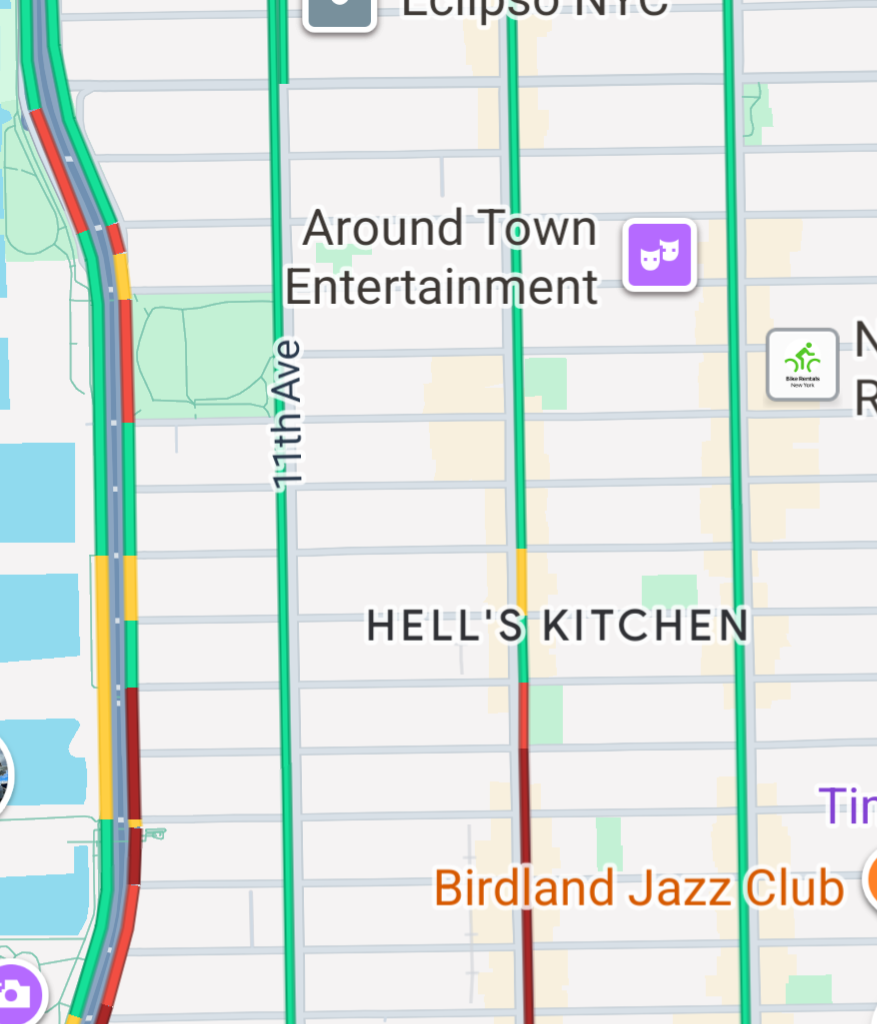
\includegraphics{../static/img/2026/manhattan}}

אז במנהטן אנחנו מודדים מרחקים על ידי הקו הישר בין שתי נקודות, כי אי
אפשר ללכת בקו הישר הזה, אלא באורך המסלול הקצר ביותר בין שתי נקודות
שבו הולכים רק ימינה/שמאלה ולמעלה/למטה. במנהטן האמיתית יש עוד מגבלה
כי אי אפשר להתחיל ללכת בכיוון מסוים מתי שרוצים, צריך להגיע להצטלבות,
אבל בואו נשמור את העניינים פשוטים יחסית. אז בשיטת המדידה החדשה הזו,
מה המרחק בין שתי נקודות, \L{$p_{1}=\left(x_{1},y_{1}\right)$} ו-\L{$p_{2}=\left(x_{2},x_{2}\right)$}?
הוא יהיה

\L{$d_{1}\left(p_{1},p_{2}\right)=\left|x_{2}-x_{1}\right|+\left|y_{2}-y_{1}\right|$}

כי \L{$\left|x_{2}-x_{1}\right|$} הוא כמה צריך ללכת ימינה/שמאלה ו-\L{$\left|y_{2}-y_{1}\right|$}
הוא כמה צריך ללכת למעלה/למטה. וגם את זה אפשר לעשות ב-\L{$n$} ממדים:

\L{$d_{1}\left(a,b\right)=\sum^{n}_{i=1}\left|b_{i}-a_{i}\right|$}

בואו נשווה את זה למטריקה הקודמת שראיתי, שעכשיו אסמן עם \L{$d_{2}$}:

\L{$d_{2}\left(a,b\right)=\sqrt{\sum^{n}_{i=1}\left(b_{i}-a_{i}\right)^{2}}$}

זה לא נראה \textbf{כל כך} דומה אבל גם לא כל כך שונה - בשני המקרים
יש לנו סכום שמערב הפרשים של זוגות של קואורדינטות. תנו לי לכתוב את
זה מחדש בצורה שקולה עבור שני המקרים אבל שבה הדמיון יהיה יותר ברור:

\L{$d_{1}\left(a,b\right)=\sqrt[1]{\sum^{n}_{i=1}\left|b_{i}-a_{i}\right|}$}

\L{$d_{2}\left(a,b\right)=\sqrt[2]{\sum^{n}_{i=1}\left|b_{i}-a_{i}\right|^{2}}$}

זה שקול למה שראינו קודם, כי \L{$\sqrt[1]{x}$} זו דרך טיפשית לכתוב
\L{$x$}, וכי \L{$\left(b_{i}-a_{i}\right)^{2}=\left|b_{i}-a_{i}\right|^{2}$}
כי ככה העלאה בריבוע עובדת, גם אם מה שמועלה בריבוע היה שלילי נקבל את
אותה התוצאה כאילו העלנו בריבוע את הערך המוחלט שלו.

האם אפשר להכליל את זה? כן! זה עובד לכל \L{$1\le p$}, אפילו אם \L{$p$}
הוא בכלל לא מספר טבעי. אפשר להגדיר פונקציה

\L{$d_{p}\left(a,b\right)=\sqrt[p]{\sum^{n}_{i=1}\left|b_{i}-a_{i}\right|^{p}}$}

והתוצאה תהיה מטריקה. וזה מעורר עוד שאלה אוטומטית אצל מתמטיקאים: מה
קורה אם לוקחים את זה לגבול? כלומר, יש לנו פה סדרה של פונקציות שתלויה
בפרמטר \L{$p$}, לאיזו פונקציה זה שואף כשמשאיפים את \L{$p$} לאינסוף?
התוצאה היא המטריקה הפשוטה יחסית הזו:

\L{$d_{\infty}\left(a,b\right)=\max\left\{ \left|b_{i}-a_{i}\right|\ |\ 1\le i\le n\right\} $}

כלומר, במטריקה הזו אנחנו צריכים ללכת רק בציר אחד, שבו המרחק הוא הארוך
ביותר; את השאר אנחנו מקבלים ב\textquotedblright חינם\textquotedblright .
לי אישית זה נשמע מוזר ממבט ראשון שזו תהיה מטריקה, ולכן זה תרגיל נחמד
לנסות להוכיח שכל התכונות של מטריקה מתקיימות גם כאן.

דרך מצויינת לקבל אינטואיציה לגבי המטריקות הללו היא פשוט לצייר את כדור
היחידה במישור. המילה \textbf{כדור} אצלי באה לתאר את קבוצת כל הנקודות
שהמרחק שלהם מנקודה נתונה \L{$a$} קטן מרדיוס מסוים \L{$r$}, מה שבדרך
כלל נקרא \textbf{עיגול} כשמדברים על המישור; אבל אני הולך להשתמש ב\textquotedblright כדור\textquotedblright{}
בהרבה הקשרים מלבד המישור אז בואו נשתמש בשם המקובל כבר מההתחלה. פורמלית,
בכל מרחב מטרי \L{$\left(X,d\right)$} אם יש לי נקודה \L{$a\in X$}
ומספר ממשי \L{$r\ge0$} אז \textbf{הכדור הפתוח} מרדיוס \L{$r$} סביב
\L{$a$} הוא הקבוצה

\L{$B\left(a,r\right)=\left\{ x\in X\ |\ d\left(a,x\right)<r\right\} $}

ב-\L{$\mathbb{R}$} עם המרחק הרגיל, \textquotedblleft הכדור הפתוח
מרדיוס \L{$\varepsilon>0$}\textquotedblright{} סביב \L{$a$} הוא הקטע
הפתוח \L{$\left(a-\varepsilon,a+\varepsilon\right)$}, וזו אחת הקבוצות
השימושיות ביותר כשמתחילים ללמוד חשבון אינפיניטסימלי כי, ובכן, בואו
ניזכר בהגדרת הגבול שהראתי בתחילת הפוסט:
\begin{itemize}
\item לכל \L{$\varepsilon>0$} קיים \L{$N>0$} כך שלכל \L{$n>N$} מתקיים
\L{$\left|a_{n}-a\right|<\varepsilon$}
\end{itemize}
את הקריטריון \L{$\left|a_{n}-a\right|<\varepsilon$} אפשר לנסח גם
בתור \L{$a_{n}\in\left(a-\varepsilon,a+\varepsilon\right)$}, ואפשר
גם להשתמש ישירות בטרמינולוגיה ובסימונים של \textquotedblleft כדור\textquotedblright :
\begin{itemize}
\item לכל \L{$\varepsilon>0$} קיים \L{$N>0$} כך שלכל \L{$n>N$} מתקיים
\L{$a_{n}\in B\left(a,\varepsilon\right)$}
\end{itemize}
זה שינוי קטנטן לכאורה, אבל הוא מעניין כי הוא מקטין את רמת ה\textquotedblright קטנוניות\textquotedblright{}
של ההגדרה: אנחנו כבר לא עושים באופן מפורש פעולה חשבונית כלשהי שמערבת
את \L{$a,a_{n}$} אלא אנחנו מסתכלים על \textquotedblleft המרחב\textquotedblright{}
ועל תתי-קבוצות מעניינות שלו. כמובן, יש פה עדיין סוג של קטנוניות -
אנחנו עדיין מסתכלים על קבוצה עם צורה מאוד ספציפית, של מרחק קונקרטי
מנקודה מסויימת קונקרטית; בהמשך נראה שאפשר גם להיפטר מזה.

עכשיו, איך נראה הכדור מרדיוס {\beginL 1\endL} סביב ראשית הצירים ב-\L{$\mathbb{R}^{2}$}
במטריקות השונות שראינו? ככה:

\L{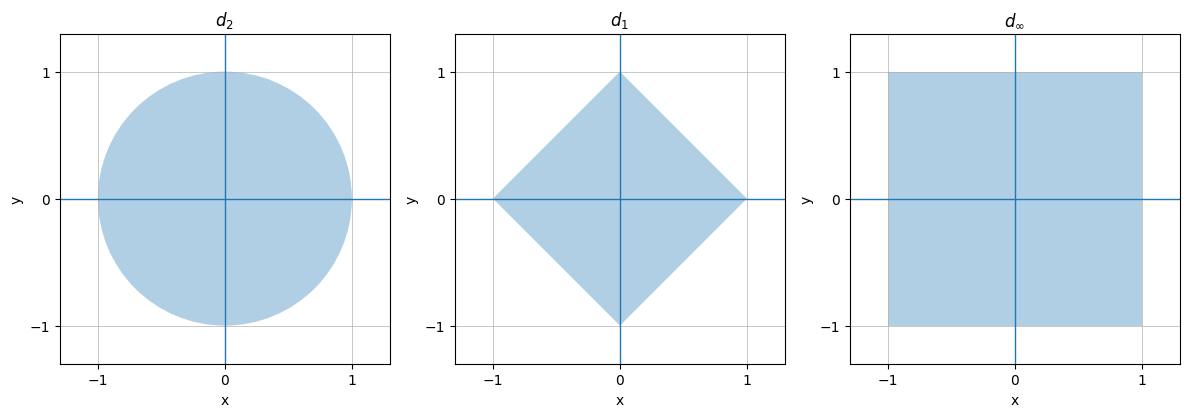
\includegraphics{../static/img/2026/unit_balls}}

ב-\L{$d_{2}$} זה עיגול \textquotedblleft רגיל\textquotedblright .
ב-\L{$d_{1}$} זה פתאום הופך למין יהלום, וב-\L{$d_{\infty}$} זה ריבוע
\textquotedblleft רגיל\textquotedblright . למה? ב-\L{$d_{1}$}, קו
הגבול של הכדור הוא כל הנקודות \L{$\left(x,y\right)$} שמרחקן מ-\L{$\left(0,0\right)$}
הוא \L{$1$}, כלומר שמקיימות \L{$\left|x\right|+\left|y\right|=1$}.
ברביע הראשון שבו \L{$x,y\ge0$}, המשוואה של הקו הזה היא פשוט \L{$x+y=1$},
שאפשר גם לכתוב בתור \L{$y=1-x$}. כלומר - זה קו ישר, עם שיפוע \L{$-1$},
שעובר דרך הנקודות \L{$\left(0,1\right)$} ו-\L{$\left(1,0\right)$}.
זה בדיוק הקו האלכסוני שבאיור, ושיקולי סימטריה מראים שגם יתר הגבולות
של הכדור צריכים להיראות ככה.

ב-\L{$d_{\infty}$} הסיפור קצת שונה - כאן קו הגבול הוא כל הנקודות
\L{$\left(x,y\right)$} שבהן או \L{$x$} או \L{$y$} הם {\beginL 1\endL}
בערכם המוחלט והשני לא גדול מ-{\beginL 1\endL}. כלומר, למשל יש את הקו
של כל הנקודות מהצורה \L{$\left(1,y\right)$} כך ש-\L{$-1\le y\le1$}
והקו \L{$\left(x,1\right)$} כך ש-\L{$-1\le x\le1$} וכדומה - קווים
אופקיים ואנכיים, כמו באיור.

זה מסיים את השאלה המקורית שלנו, \textquotedblleft מה זה מרחבים מטריים\textquotedblright .
עכשיו אפשר לעבור לשאלה הבאה, \textquotedblleft ואיך אפשר להיפטר מהם\textquotedblright ,
כלומר - מה התכונות של מרחבים מטריים שנוכל להכליל הלאה ועדיין להישאר
עם היכולת לתאר שלל דברים שמעניינים אותנו. את זה נראה בפוסט הבא. כמו
שהבטחתי, נתחיל מלדבר על קבוצות פתוחות.
\end{document}
